\begin{figure}[t]
    \begin{minipage}[t]{.45\textwidth}
       \begin{center}
    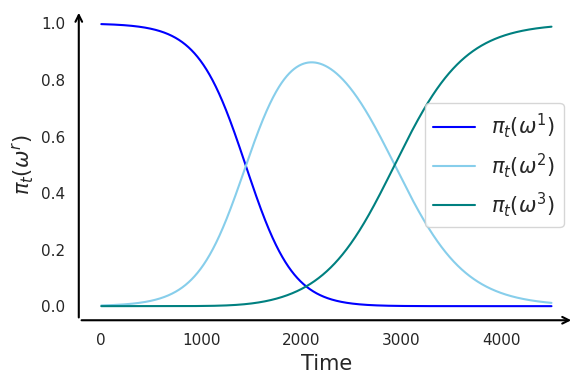
\includegraphics[width=0.9\textwidth]{figures/alignement_plot.png}
  \end{center}
  \vspace{-10pt}
   \caption{Illustration of $\pi_t\left(\boldsymbol{\omega}^r\right)$ after Fantom's first iteration with equal windows of 1500 samples for an MTS of 4500 samples with two ground-truth regimes: $\mathcal{I}^{*}_1 = [|0:1999|]$ and $\mathcal{I}^{*}_2 = [|2000:4500|]$.}
  \vspace{-10pt}
    \end{minipage}
    \hfill
    \begin{minipage}[t]{.45\textwidth}
        \begin{center}
    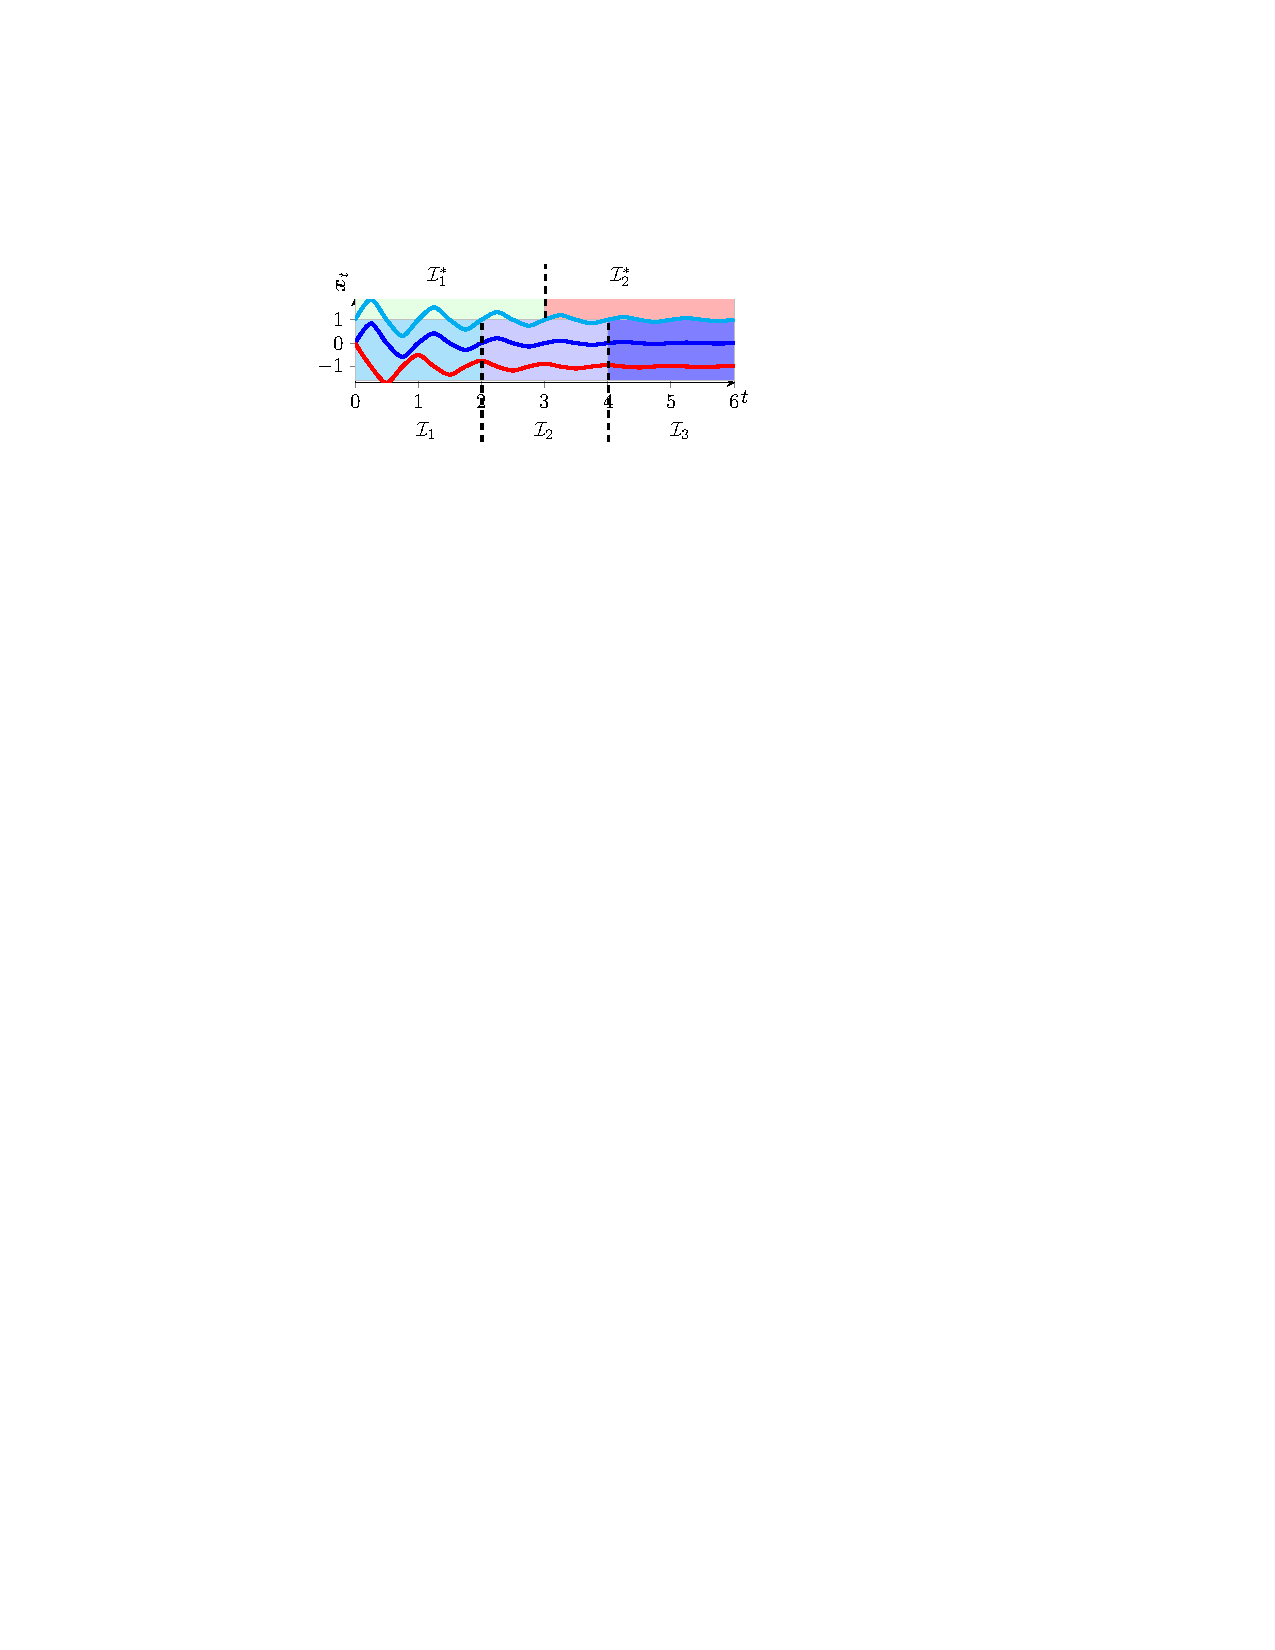
\includegraphics[width=0.9\textwidth]{figures/tikz_Neurips.pdf}
\end{center}
  \vspace{-15pt}
  \caption{Example of initialization with $N_w=3$ windows, $\mathcal{I}_1$ and $\mathcal{I}_3$ are pure regimes while $\mathcal{I}_2$ is impure (composed of samples from two ground-truth regimes $\mathcal{I}_1^*$ and $\mathcal{I}_2^*, K=2$ ).}
  \label{pure_impure_fig}
  %\vspace{-20pt} 
    \end{minipage}  
    %\label{fig:1-2}
    %\caption{Title.}
\end{figure}
\begin{equation*}
\begin{aligned}
\textcolor{black}{\beta^r_{t}} & =p\left(z_{r}=1 \mid \boldsymbol{x}_t,\boldsymbol{x}_{<t}, \boldsymbol{G}^{r}_{\{0: L\}}\right) \\
& \textcolor{black}{=\frac{p\left(z_{t}=r\right) p\left(\boldsymbol{x}_t \mid \boldsymbol{x}_{<t}, z_{t}=r, \mathcal{G}^r\right)}{\sum_{j=1}^{N_w} p\left(z_{t}=j\right) p\left(\boldsymbol{x}_t \mid \boldsymbol{x}_{<t}, z_{t}=j, \mathcal{G}^j\right)}} \\
& \textcolor{black}{\propto \pi_t(\boldsymbol{\omega}^{r}) p\left(\boldsymbol{x}_t \mid \boldsymbol{x}_{<t}, z_{t}=r, \mathcal{G}^r\right)},
\end{aligned}
\end{equation*}
where $p(\boldsymbol{x}_t \mid \boldsymbol{x}_{<t}, z_{t} = r, \mathcal{G}^r)$ denotes the likelihood of $\boldsymbol{x}_t$ being generated by the SEM from Equation~(\ref{eq_multi_reg_hetero}) for regime $r$. This probability is computed using the normalizing flows trained during the M-step, following the same reasoning as in Eq(\ref{proba_nf_math}).

The probability of $\boldsymbol{x}_t$ belonging to regime $r$ is influenced by two main factors: the observation’s position within its current regime and whether that regime is designated as \textcolor{RoyalBlue}{pure or impure}. In order to clarify the intuition behind \textcolor{RoyalBlue}{pure and impure} regimes, Figure \ref{pure_impure_fig} shows an example of such case. It presents an initialization of three equal windows while the MTS is composed of two ground truth regimes presented by green color $\mathcal{I}_{1}^*$ and red one $\mathcal{I}_{2}^*$. In such case, the regimes $\mathcal{I}_1$ and $\mathcal{I}_3$ are pure, because they are composed of samples coming from the same ground truth regime ($\mathcal{I}_{1}^*$ for the regime $\mathcal{I}_1$ and $\mathcal{I}_{2}^*$ for the regime $\mathcal{I}_3$), while $\mathcal{I}_2$ is an impure regime and has samples from the two ground truth regimes.

We highlight all the different cases for a sample $\boldsymbol{x}_t$ either near to the border or not of regime $r$ and also either the causal graph learned for $r$ is on \textcolor{RoyalBlue}{pure or impure} data:

\textbf{Case 1:}  
If $\boldsymbol{x}_t$ is in a \textcolor{RoyalBlue}{pure} regime $r$ and is far from the boundary in the current iteration, $\pi_t(\boldsymbol{\omega}^r)$ takes a high value (for example, $\pi_{t \in [0,1000]}(\boldsymbol{\omega}^1)$ in Figure~\ref{fig:pi_alignement}). Because regime $r$ was trained on pure data, its causal graph is more accurate, leading to a high likelihood $p(\boldsymbol{x}_t \mid \boldsymbol{x}_{<t},\, z_t = r,\, \mathcal{G}^r)$. Consequently,
$
\beta_t^r \propto \pi_t(\boldsymbol{\omega}^r)\; p(\boldsymbol{x}_t \mid \boldsymbol{x}_{<t},\, z_t = r,\, \mathcal{G}^r)
$
remains dominant, causing $\boldsymbol{x}_t$ to stay in regime $r$ at the next iteration.

\textbf{Case 2:}  
If $\boldsymbol{x}_t$ is in a \textcolor{RoyalBlue}{pure} regime $r$ but is near the boundary in the current iteration, $\pi_t(\boldsymbol{\omega}^r)$ and $\pi_t(\alpha_{u+1})$ are nearly equal (e.g., $\pi_{t \in [1100,1500]}(\boldsymbol{\omega}^1)$ vs.\ $\pi_{t \in [1100,1500]}(\boldsymbol{\omega}^2)$ in Figure~\ref{fig:pi_alignement})). Nonetheless, since regime $r$ was learned from pure data, $p(\boldsymbol{x}_t \mid \boldsymbol{x}_{<t}, z_t = r, \mathcal{G}^r)$ stays high, keeping $\beta_t^r$ at its maximum value and maintaining $\boldsymbol{x}_t$ in regime $r$ for the next iteration.

\textbf{Case 3:}  
If $\boldsymbol{x}_t$ is in an \textcolor{RoyalBlue}{impure} regime $r+1$ near the boundary during the current iteration, $\pi_t(\boldsymbol{\omega}^r)$ and $\pi_t(\boldsymbol{\omega}^{r+1})$ are also close in value (e.g., $\pi_{t \in [1501,1800]}(\boldsymbol{\omega}^1)$ vs.\ $\pi_{t \in [1501,1800]}(\boldsymbol{\omega}^2)$ in Figure \ref{fig:pi_alignement}). However, because the causal graph for regime $r$ is more reliable (having been derived from pure data),
$
p(\boldsymbol{x}_t \mid \boldsymbol{x}_{<t}, z_t = r, \mathcal{G}^r)
>
p(\boldsymbol{x}_t \mid  \boldsymbol{x}_{<t}, z_t = r+1, \mathcal{G}^{r+1}).
$
As a result, $\boldsymbol{x}_t$ moves from regime $r+1$ to $r$ in the next iteration.

\textbf{Case 4:}
$\boldsymbol{x}_t$ belongs to impure regime $r+1$ and is far from the border (e.g., $t \in [1801,2500]$ in Figure \ref{fig:pi_alignement}). In this case, it's uncertain whether $\boldsymbol{x}_t$ will switch regimes in the next iteration. However, as the pure regime $r$ expands with each iteration, $\boldsymbol{x}_t$ will eventually be near the border of regime $r+1$, bringing us back to Case~3.